\documentclass{standalone}
\usepackage{tikz}
\usetikzlibrary{positioning}

\begin{document}

    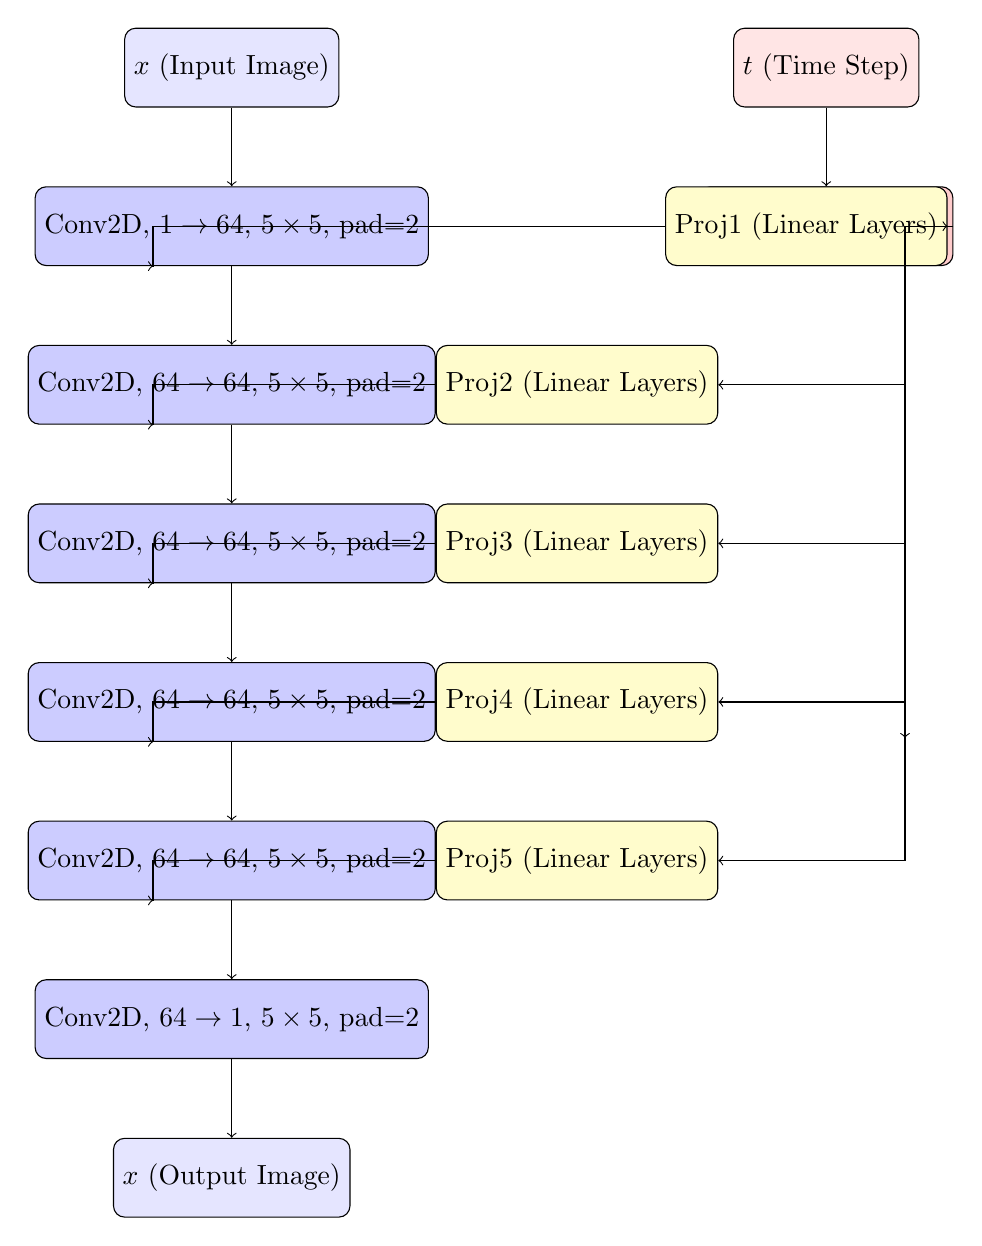
\begin{tikzpicture}

        % Input tensors
        \node[draw, rounded corners, fill=blue!10, minimum width=2cm, minimum height=1cm] (input_x) at (0,0) {$x$ (Input Image)};
        \node[draw, rounded corners, fill=red!10, minimum width=2cm, minimum height=1cm, right=5cm of input_x] (input_t) {$t$ (Time Step)};

        % Embedding layer
        \node[draw, rounded corners, fill=red!20, minimum width=3cm, minimum height=1cm, below=1cm of input_t] (embed) {Embedding, $t \to 64$};

        % Convolution layers with detailed values
        \node[draw, rounded corners, fill=blue!20, minimum width=3.5cm, minimum height=1cm, below=1cm of input_x] (conv1) {Conv2D, $1 \to 64$, $5 \times 5$, pad=2};
        \node[draw, rounded corners, fill=blue!20, minimum width=3.5cm, minimum height=1cm, below=1cm of conv1] (conv2) {Conv2D, $64 \to 64$, $5 \times 5$, pad=2};
        \node[draw, rounded corners, fill=blue!20, minimum width=3.5cm, minimum height=1cm, below=1cm of conv2] (conv3) {Conv2D, $64 \to 64$, $5 \times 5$, pad=2};
        \node[draw, rounded corners, fill=blue!20, minimum width=3.5cm, minimum height=1cm, below=1cm of conv3] (conv4) {Conv2D, $64 \to 64$, $5 \times 5$, pad=2};
        \node[draw, rounded corners, fill=blue!20, minimum width=3.5cm, minimum height=1cm, below=1cm of conv4] (conv5) {Conv2D, $64 \to 64$, $5 \times 5$, pad=2};
        \node[draw, rounded corners, fill=blue!20, minimum width=3.5cm, minimum height=1cm, below=1cm of conv5] (conv6) {Conv2D, $64 \to 1$, $5 \times 5$, pad=2};

        % Projection layers with staggered positioning
        \node[draw, rounded corners, fill=yellow!20, minimum width=3.5cm, minimum height=1cm, right=3cm of conv1] (proj1) {Proj1 (Linear Layers)};
        \node[draw, rounded corners, fill=yellow!20, minimum width=3.5cm, minimum height=1cm, below=1cm of proj1, right=0cm of conv2] (proj2) {Proj2 (Linear Layers)};
        \node[draw, rounded corners, fill=yellow!20, minimum width=3.5cm, minimum height=1cm, below=1cm of proj2, right=0cm of conv3] (proj3) {Proj3 (Linear Layers)};
        \node[draw, rounded corners, fill=yellow!20, minimum width=3.5cm, minimum height=1cm, below=1cm of proj3, right=0cm of conv4] (proj4) {Proj4 (Linear Layers)};
        \node[draw, rounded corners, fill=yellow!20, minimum width=3.5cm, minimum height=1cm, below=1cm of proj4, right=0cm of conv5] (proj5) {Proj5 (Linear Layers)};

        % Output tensor
        \node[draw, rounded corners, fill=blue!10, minimum width=2cm, minimum height=1cm, below=1cm of conv6] (output) {$x$ (Output Image)};

        % Draw connections
        \draw[->] (input_x) -- (conv1);
        \draw[->] (conv1) -- (conv2);
        \draw[->] (conv2) -- (conv3);
        \draw[->] (conv3) -- (conv4);
        \draw[->] (conv4) -- (conv5);
        \draw[->] (conv5) -- (conv6);
        \draw[->] (conv6) -- (output);

        % Embedding and branching connections to projection layers
        \draw[->] (input_t) -- (embed);
        \draw[->] (embed) -- ++(1,0) coordinate (branch) -- ++(0,-6.5) coordinate (line_end);
        \draw[->] (branch) |- (proj1);
        \draw[->] (branch) |- (proj2);
        \draw[->] (branch) |- (proj3);
        \draw[->] (branch) |- (proj4);
        \draw[->] (branch) |- (proj5);

        % Projection layers to convolution layers
        \draw[->] (proj1) -| ([xshift=-1cm]conv1.south) -- (conv1);
        \draw[->] (proj2) -| ([xshift=-1cm]conv2.south) -- (conv2);
        \draw[->] (proj3) -| ([xshift=-1cm]conv3.south) -- (conv3);
        \draw[->] (proj4) -| ([xshift=-1cm]conv4.south) -- (conv4);
        \draw[->] (proj5) -| ([xshift=-1cm]conv5.south) -- (conv5);

    \end{tikzpicture}

\end{document}
